\documentclass[a4paper, 14pt]{extarticle}

% Поля
%--------------------------------------
\usepackage{geometry}
\geometry{a4paper,tmargin=2cm,bmargin=2cm,lmargin=3cm,rmargin=1cm}
%--------------------------------------


%Russian-specific packages
%--------------------------------------
\usepackage[T2A]{fontenc}
\usepackage[utf8]{inputenc} 
\usepackage[english, main=russian]{babel}
%--------------------------------------

\usepackage{textcomp}

% Красная строка
%--------------------------------------
\usepackage{indentfirst}               
%--------------------------------------             


%Graphics
%--------------------------------------
\usepackage{graphicx}
\graphicspath{ {./images/} }
\usepackage{wrapfig}
%--------------------------------------

% Полуторный интервал
%--------------------------------------
\linespread{1.3}                    
%--------------------------------------

%Выравнивание и переносы
%--------------------------------------
% Избавляемся от переполнений
\sloppy
% Запрещаем разрыв страницы после первой строки абзаца
\clubpenalty=10000
% Запрещаем разрыв страницы после последней строки абзаца
\widowpenalty=10000
%--------------------------------------

%Списки
\usepackage{enumitem}

%Подписи
\usepackage{caption} 

%Гиперссылки
\usepackage{hyperref}

\hypersetup {
	unicode=true
}

%Рисунки
%--------------------------------------
\DeclareCaptionLabelSeparator*{emdash}{~--- }
\captionsetup[figure]{labelsep=emdash,font=onehalfspacing,position=bottom}
%--------------------------------------

\usepackage{tempora}

%Листинги
%--------------------------------------
\usepackage{listings}
\lstset{
  basicstyle=\ttfamily\footnotesize, 
  %basicstyle=\footnotesize\AnkaCoder,        % the size of the fonts that are used for the code
  breakatwhitespace=false,         % sets if automatic breaks shoulbd only happen at whitespace
  breaklines=true,                 % sets automatic line breaking
  captionpos=t,                    % sets the caption-position to bottom
  inputencoding=utf8,
  frame=single,                    % adds a frame around the code
  keepspaces=true,                 % keeps spaces in text, useful for keeping indentation of code (possibly needs columns=flexible)
  keywordstyle=\bf,       % keyword style
  numbers=left,                    % where to put the line-numbers; possible values are (none, left, right)
  numbersep=5pt,                   % how far the line-numbers are from the code
  xleftmargin=25pt,
  xrightmargin=25pt,
  showspaces=false,                % show spaces everywhere adding particular underscores; it overrides 'showstringspaces'
  showstringspaces=false,          % underline spaces within strings only
  showtabs=false,                  % show tabs within strings adding particular underscores
  stepnumber=1,                    % the step between two line-numbers. If it's 1, each line will be numbered
  tabsize=2,                       % sets default tabsize to 8 spaces
  title=\lstname                   % show the filename of files included with \lstinputlisting; also try caption instead of title
}
%--------------------------------------

%%% Математические пакеты %%%
%--------------------------------------
\usepackage{amsthm,amsfonts,amsmath,amssymb,amscd}  % Математические дополнения от AMS
\usepackage{mathtools}                              % Добавляет окружение multlined
\usepackage[perpage]{footmisc}
%--------------------------------------

%--------------------------------------
%			НАЧАЛО ДОКУМЕНТА
%--------------------------------------

\begin{document}

%--------------------------------------
%			ТИТУЛЬНЫЙ ЛИСТ
%--------------------------------------
\begin{titlepage}
\thispagestyle{empty}
\newpage


%Шапка титульного листа
%--------------------------------------
\vspace*{-60pt}
\hspace{-65pt}
\begin{minipage}{0.3\textwidth}
\hspace*{-20pt}\centering

\includegraphics[width=\textwidth]{emblem}
\end{minipage}
\begin{minipage}{0.67\textwidth}\small \textbf{
\vspace*{-0.7ex}
\hspace*{-6pt}\centerline{Министерство науки и высшего образования Российской Федерации}
\vspace*{-0.7ex}
\centerline{Федеральное государственное бюджетное образовательное учреждение }
\vspace*{-0.7ex}
\centerline{высшего образования}
\vspace*{-0.7ex}
\centerline{<<Московский государственный технический университет}
\vspace*{-0.7ex}
\centerline{имени Н.Э. Баумана}
\vspace*{-0.7ex}
\centerline{(национальный исследовательский университет)>>}
\vspace*{-0.7ex}
\centerline{(МГТУ им. Н.Э. Баумана)}}
\end{minipage}
%--------------------------------------

%Полосы
%--------------------------------------
\vspace{-25pt}
\hspace{-35pt}\rule{\textwidth}{2.3pt}

\vspace*{-20.3pt}
\hspace{-35pt}\rule{\textwidth}{0.4pt}
%--------------------------------------

\vspace{1.5ex}
\hspace{-35pt} \noindent \small ФАКУЛЬТЕТ\hspace{80pt} <<Информатика и системы управления>>

\vspace*{-16pt}
\hspace{47pt}\rule{0.83\textwidth}{0.4pt}

\vspace{0.5ex}
\hspace{-35pt} \noindent \small КАФЕДРА\hspace{50pt} <<Теоретическая информатика и компьютерные технологии>>

\vspace*{-16pt}
\hspace{30pt}\rule{0.866\textwidth}{0.4pt}
  
\vspace{11em}

\begin{center}
\Large {\bf Лабораторная работа № 7} \\ 
\large {\bf по курсу <<Языки и методы программирования>>} \\
\large <<Разработка простейшего класса на C++>> 
\end{center}\normalsize

\vspace{8em}


\begin{flushright}
  {Студент группы ИУ9-21Б Горбунов А. Д. \hspace*{15pt}\\ 
  \vspace{2ex}
  Преподаватель Посевин Д. П.\hspace*{15pt}}
\end{flushright}

\bigskip

\vfill
 

\begin{center}
\textsl{Москва 2023}
\end{center}
\end{titlepage}
%--------------------------------------
%		КОНЕЦ ТИТУЛЬНОГО ЛИСТА
%--------------------------------------

\renewcommand{\ttdefault}{pcr}

\setlength{\tabcolsep}{3pt}
\newpage
\setcounter{page}{2}

\section{Задание}\label{Sect::task}
	Выполнение лабораторной работы заключается в составлении на языке C++
программы, состоящей из трёх файлов:
- заголовочный файл declaration.h с объявлением одного из классов, приведённых в таблицах 1 – 16;

- файл implementation.cpp с определениями методов класса;

- файл main.cpp, содержащий функцию main и, возможно, вспомогательные функции для проверки работоспособности класса.

Реализация класса не должна опираться на стандартные контейнерные классы
C++, то есть внутреннее состояние объектов класса должно быть реализовано через обычные массивы. Соответственно, в классе обязательно требуется реализовать:

- конструктор копий;

- деструктор (должен быть объявлен виртуальным);

- операцию присваивания.

Проверку работоспособности класса требуется организовать в функции main, размещённой в файле main.cpp.

Проверка должна включать в себя:

- создание объекта класса в автоматической памяти;

- передачу объекта класса по значению в функцию;

- присваивание объекта класса переменной.


    Доска для игры в крестики-нолики размером n ×
n с операциями:
1. получение размера доски;
2. получение ссылки на клетку с указанными
координатами;
3. определение, является ли текущая позиция
финальной.
\section{Результаты}\label{Sect::res}

Исходный код программы представлен в листинге~\ref{lst:code1}, ~\ref{lst:code2}, ~\ref{lst:code3}

\begin{figure}[!htb]
\begin{lstlisting}[language={},caption={main.cpp},label={lst:code1}]
#include <iostream>
#include "TicTacToeBoard.h"
using namespace std;
int main() {
    int n = 3;
    TicTacToeBoard board(n);
    board.getCell(0, 0) = 'X';
    board.getCell(0, 0) = 'O';
    board.getCell(1, 1) = 'O';
    board.getCell(0, 2) = 'O';
    board.getCell(2, 2) = 'X';
    cout << "Size: " << board.getSize() << endl;
    cout << "Cell (0, 0): " << board.getCell(0, 0) << endl;
    cout << "Cell (1, 1): " << board.getCell(1, 1) << endl;
    cout << "Is final position: " << board.isFinalPosition() << endl;
    return 0;
}
\end{lstlisting}
\end{figure}

\begin{figure}[!htb]
\begin{lstlisting}[language={},caption={класс TicTacToeBoard},label={lst:code2}]
class TicTacToeBoard {
private:
    char **board;
    int size;
public:
    TicTacToeBoard(int n) {
        size = n;
        board = new char*[size];
        for (int i = 0; i < size; i++) {
            board[i] = new char[size];
            for (int j = 0; j < size; j++) {
                board[i][j] = '_';
            }
        }
    }
    int getSize() {
        return size;
    }
    char &getCell(int i, int j) {
        return board[i][j];
    }
    bool isFinalPosition() {
        for (int i = 0; i < size; i++) {
            int j = 0;
            while (j < size - 1 && board[i][j] == board[i][j + 1]) {
                j++;
            }
            if (j == size - 1 && board[i][j] != '_') {
                return true;
            }
        }
\end{lstlisting}
\end{figure}

\begin{figure}[!htb]
\begin{lstlisting}[language={},caption={класс TicTacToeBoard(продолжение)},label={lst:code3}]
        for (int j = 0; j < size; j++) {
            int i = 0;
            while (i < size - 1 && board[i][j] == board[i + 1][j]) {
                i++;
            }
            if (i == size - 1 && board[i][j] != '_') {
                return true;
            }
        }
        int i = 0;
        while (i < size - 1 && board[i][i] == board[i + 1][i + 1]) {
            i++;
        }
        if (i == size - 1 && board[i][i] != '_') {
            return true;
        }
        i = 0;
        while (i < size - 1 && board[i][size - i - 1] == board[i + 1][size - i - 2]) {
            i++;
        }
        if (i == size - 1 && board[i][size - i - 1] != '_') {
            return true;
        }
        for (int i = 0; i < size; i++) {
            for (int j = 0; j < size; j++) {
                if (board[i][j] == '_') {
                    return false;
                }
            }
        }
        return true;
    }
    ~TicTacToeBoard() {
        for (int i = 0; i < size; i++) {
            delete[] board[i];
        }
        delete[] board;
    }
};
\end{lstlisting}
\end{figure}

\begin{figure}[!htb]
Результат запуска представлен на рисунке ~\ref{fig:picture_1.png}, ~\ref{fig:picture_2.png}, ~\ref{fig:picture_3.png}
\end{figure}

\begin{figure}[!htb]
	\centering
	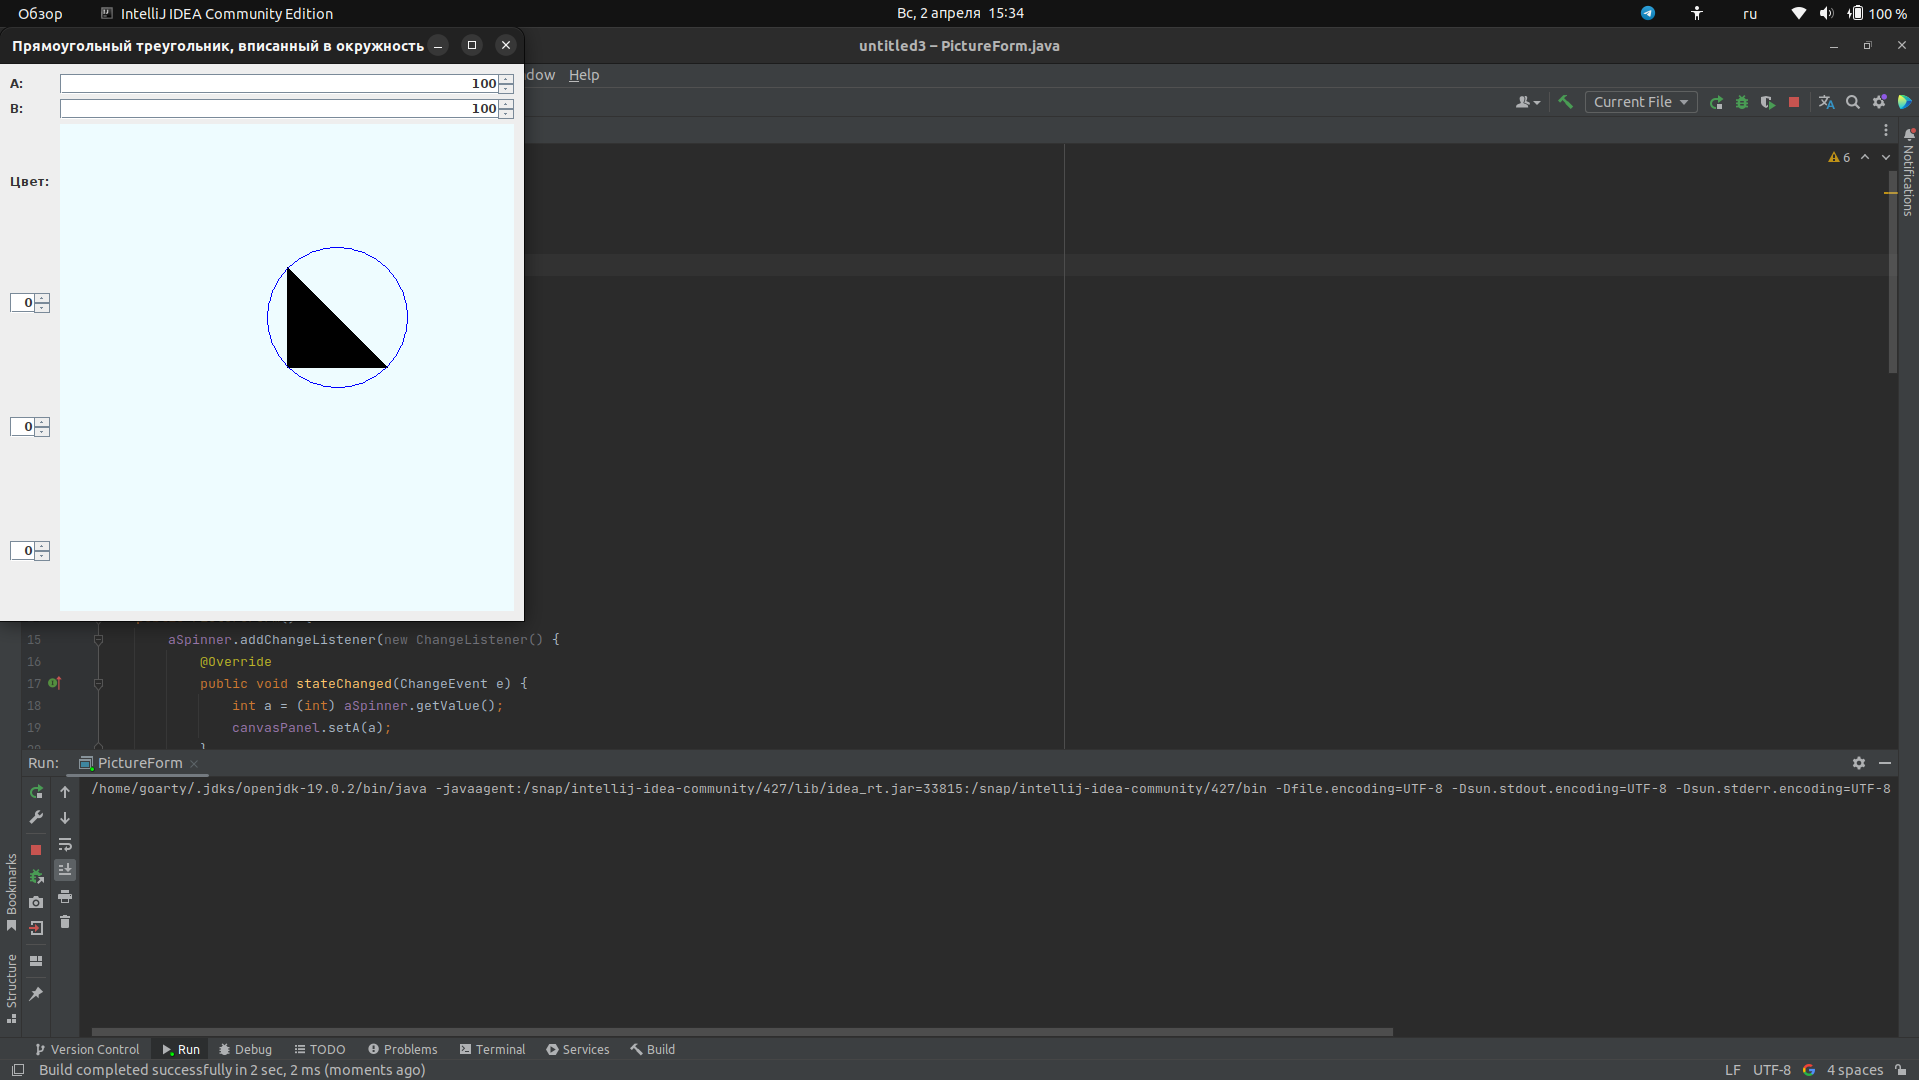
\includegraphics[width=0.8\textwidth]{picture_1.png}
\caption{Реализация main.cpp и TicTacToeBoard.h}
\label{fig:picture_1.png}
\end{figure}

\begin{figure}[!htb]
	\centering
	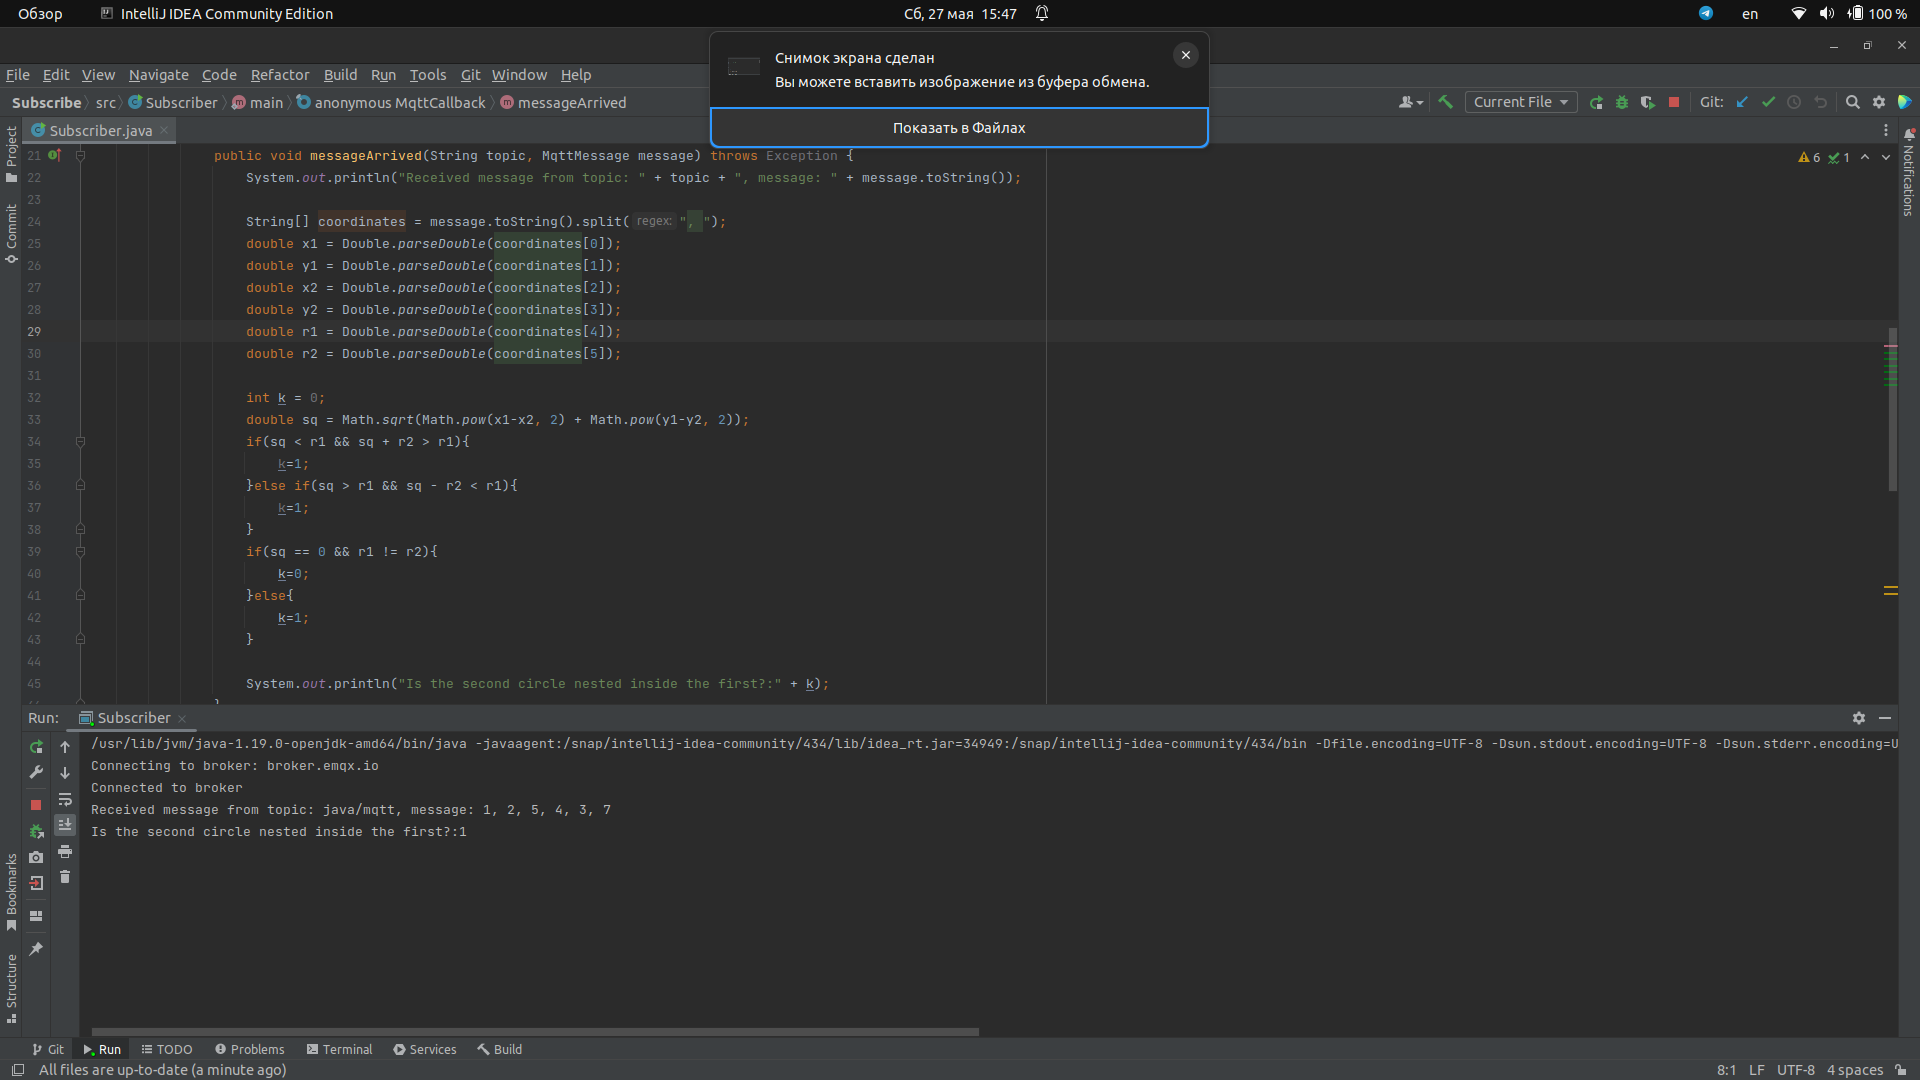
\includegraphics[width=0.8\textwidth]{picture_2.png}
\caption{Реализация main.cpp и TicTacToeBoard.h(продолжение)}
\label{fig:picture_2.png}
\end{figure}

\begin{figure}[!htb]
	\centering
	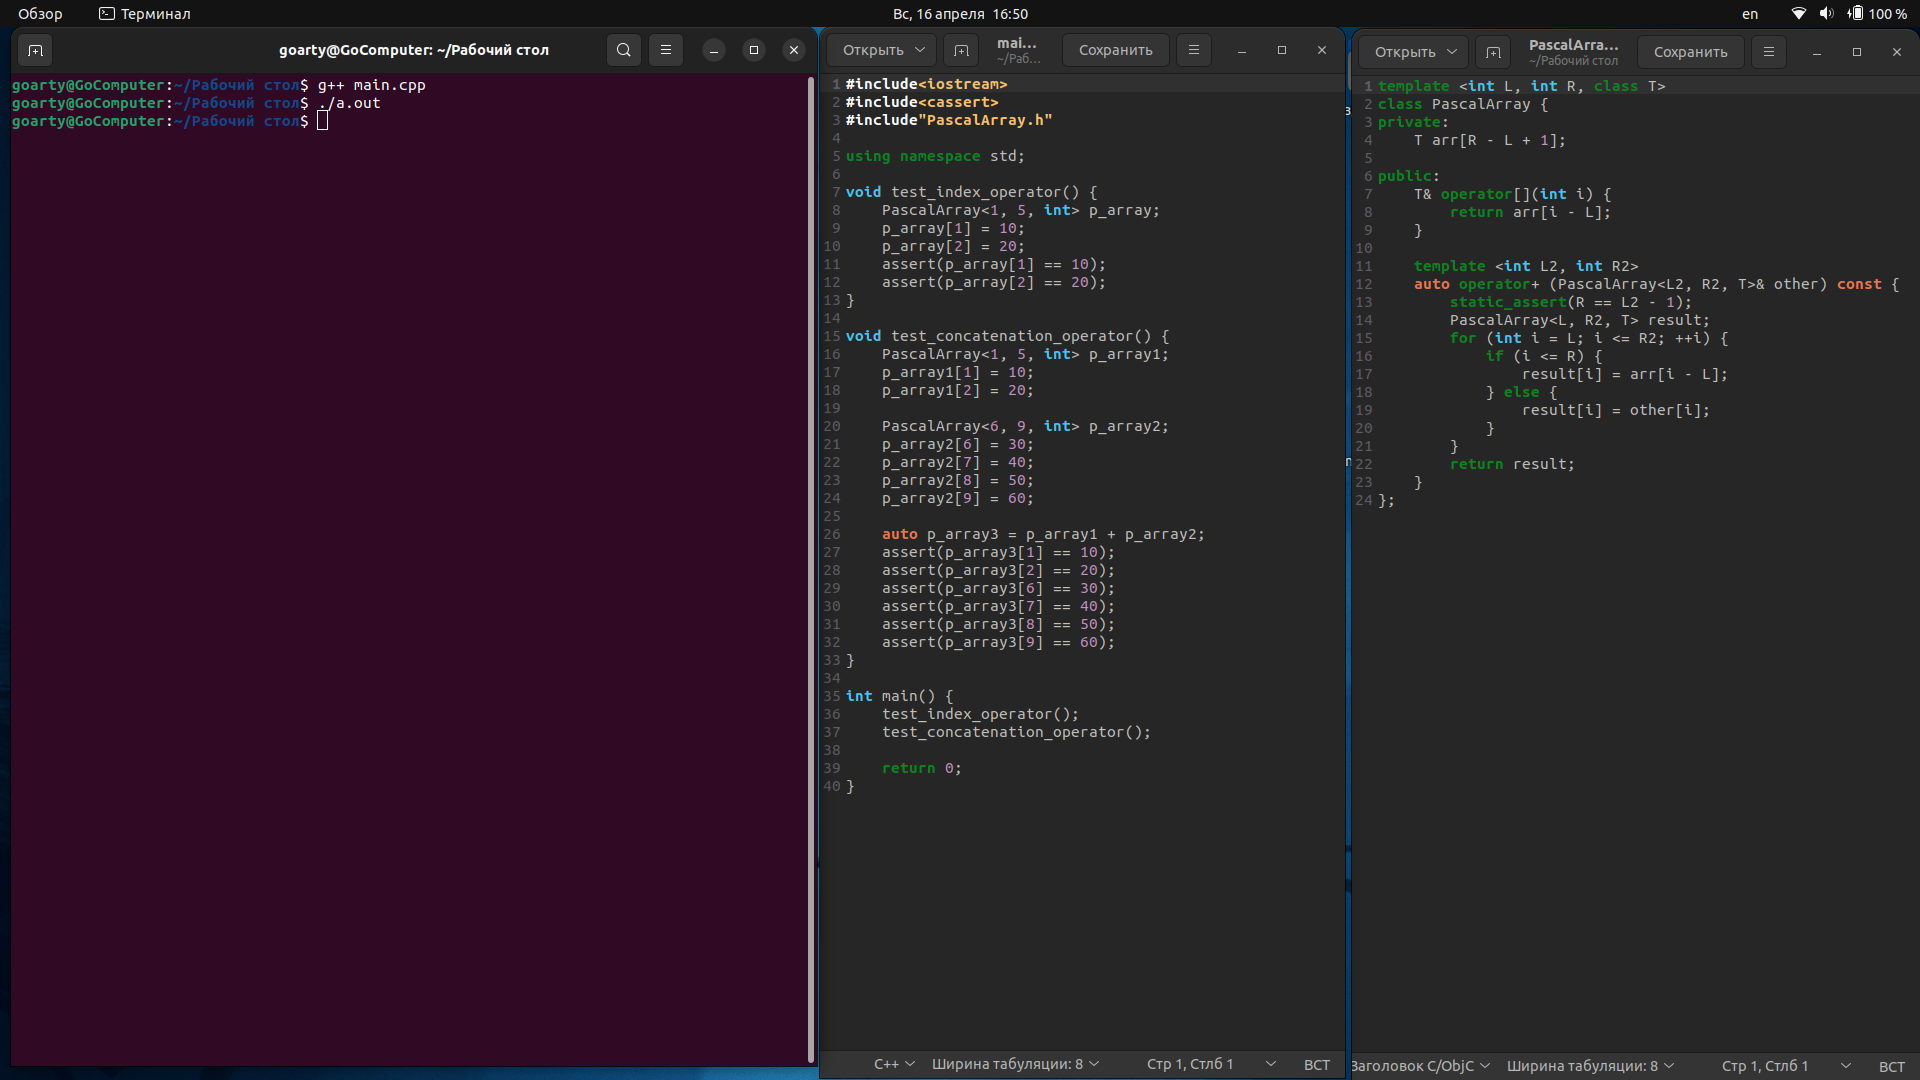
\includegraphics[width=0.8\textwidth]{picture_3.png}
\caption{Работа программы}
\label{fig:picture_3.png}
\end{figure}

\end{document}

